\documentclass[../TDE6_rsf.tex]{subfiles}%

\begin{document}
\section[s]"1"{Dipôle inconnu}
\enonce{%
	\noindent
	\begin{minipage}{0.60\linewidth}
		Dans le montage ci-contre, le GBF délivre une tension $e(t)$ sinusoïdale de
		pulsation $\w$, $R$ est une résistance et $D$ un dipôle inconnu. On note
		$u(t) = U_m\cos(\wt)$ et $v(t) = V_m\cos(\wt+\F)$ les tensions aux bornes
		respectivement de $R$ et $D$. On visualise à l'oscilloscope $v(t)$ et
		$u(t)$, et on obtient le graphe ci-dessous.
	\end{minipage}
	\begin{minipage}{0.35\linewidth}
		\begin{center}
			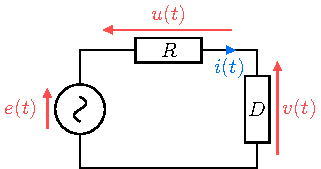
\includegraphics[width=\linewidth]{rd_rsf}
		\end{center}
	\end{minipage}

	\begin{center}
		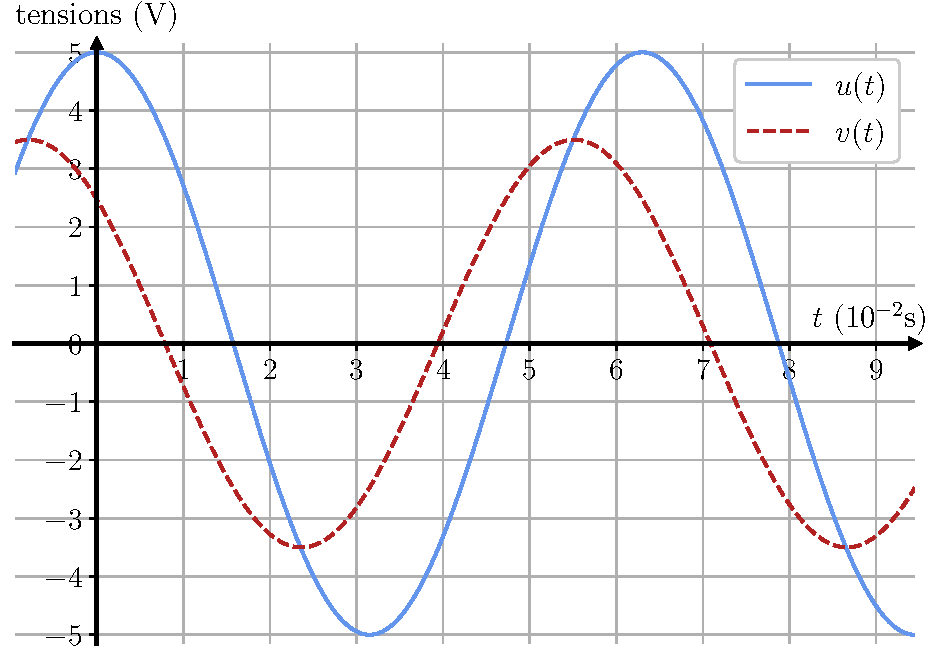
\includegraphics[scale=1]{rd_Ul_time}
	\end{center}
	On utilise ces résultats graphiques pour déterminer les
	caractéristiques de $D$, sachant que $R = \SI{100}{\Omega}$.
}

\QR{%
	Déterminer $V_m$, $U_m$ ainsi que la pulsation $\w$ des signaux
	utilisés.
}{%
	On trouve les amplitudes par lecture graphique des maxima~:
	\[
		\boxed{V_m = \SI{3.5}{V}}
		\qet
		\boxed{U_m = \SI{5}{V}}
	\]
	On fait de même pour trouver la période $T = \SI{6.3e-2}{s}$, et on en
	déduit la pulsation~:
	\[\boxed{\w = \frac{2\pi}{T} = \SI{100}{rad.s^{-1}}}\]
}

\QR{%
	La tension $v$ est-elle en avance ou en retard sur la tension $u$~? En
	déduire le signe de $\F$. Déterminer la valeur de $\F$ à partir du
	graphe.
}{%
	La tension $v$ est en $avance$ sur $u$, puisque quand $v$ s'annule en
	descendant $u$ s'annule aussi en descendant un peu plus tard que $v$. On
	peut aussi voir qu'à $t=0$, $u$ est à son maximum alors que $v$ y est
	déjà passé et est en train de diminuer. Par définition du déphasage, on
	a donc \fbox{$\D\f_{v/u} > 0$}. \bigbreak
	Or, $\D\f_{v/u} = \f_v - \f_u$ et $u(t) = U_m\cos(\wt)$ donc $\f_u = 0$.
	On trouve donc \fbox{$\F > 0$}. \bigbreak
	On a deux manières de mesurer le déphasage~:
	\begin{itemize}
		\item par définition, la pulsation est une vitesse angulaire, donc
		      une durée se convertit en phase en la multipliant par $\w$. On
		      peut donc déterminer le \textbf{déphasage} en mesurant le
		      \textbf{retard temporel} entre les deux signaux \textbf{quand
			      ils s'annulent avec la même pente}. Soit $\D t$ cet écart~: on
		      mesure
		      \begin{gather*}
			      \D t = \SI{0.75e-2}{s}
			      \Lra
			      \D\f_{v/u} = \F = \w\D t
			      \Lra
			      \boxed{\F = \SI{0.75}{rad} \approx \frac{\pi}{4}\si{rad}}
		      \end{gather*}
		\item On peut également mesurer $v(0) = V_m\cos(\F)$ et avoir
		      \begin{gather*}
			      \cos(\F) = \frac{v(0)}{V_m}
			      \Lra
			      \boxed{\F = \arccos \left( \frac{v(0)}{V_m} \right)}
			      \qavec
			      \left\{
			      \begin{array}{rcl}
				      v(0) & = & \SI{2.5}{V} \\
				      V_m  & = & \SI{3.5}{V}
			      \end{array}
			      \right.\\
			      \mathrm{A.N.~:}\quad
			      \boxed{\F \approx \SI{0.77}{rad}}
		      \end{gather*}
	\end{itemize}
}
\begin{blocQR}
	\item On note $\Zu = X + \jj Y$ l'impédance complexe du dipôle $D$.

	\QR{%
		Déterminer les valeurs de $X$ et $Y$ à partir des résultats
		précédents.
	}{%
		On nous donne $v(t)$ donc $\xul{V} = V_m\exr^{\jj\F}$, et on
		nous défini $\Zu$ son impédance. Pour faire le lien entre
		les deux, on utilise la définition de l'impédance complexe pour
		un dipôle de tension $\Uu$ et traversé par un courant
		$\xul{I}$ \textit{via} loi \textbf{loi d'Ohm généralisée}~:
		\[\boxed{\xul{V} = \Zu\xul{I}}\]
		Il faudrait donc pouvoir connaître $\xul{I}$. Heureusement, la
		loi d'\textsc{Ohm} généralisée fonction évidemment avec les
		résistances, et comme il n'y a qu'une seule intensité qui
		traverse la maille, on peut utiliser
		\[\boxed{\Uu = R\xul{I} \Lra \xul{I} =
				\frac{\Uu}{R}}\]
		Ainsi,
		\begin{gather*}
			Z = \abs{ \Zu } = \sqrt{X^2 + Y^2} \qet
			Z = \abs{ \Zu } = \abs{\frac{\xul{V}}{\xul{I}}}
			= \abs{ R\frac{\xul{V}}{\Uu} }\\
			\Lra
			\boxed{X^2 + Y^2 = R^2 \frac{V_m{}^2}{U_m{}^2}}
			\qavec
			\left\{
			\begin{array}{rcl}
				V_m & = & \SI{3.5}{V}      \\
				U_m & = & \SI{5}{V}        \\
				R   & = & \SI{100}{\Omega}
			\end{array}
			\right.\\
			\mathrm{A.N.~:}\quad
			\boxed{X^2 + Y^2 = \SI{4900}{\Omega^2}}
		\end{gather*}
		L'autre équation permettant de résoudre ce système est bien
		évidemment la phase (question 1 puis question 2)~:
		\begin{gather*}
			\tan(\arg*{\Zu}) = \frac{Y}{X} \qet \tan(\arg*{\Zu}) =
			\tan\big(\arg*{\xul{V}} -
			\underbracket[1pt]{\cancel{\arg*{\Uu}}}_{=0}\big) = \tan(\F)\\
			\Lra
			\frac{Y}{X} = \tan\F
			\qavec
			\F = \frac{\pi}{4}\si{rad}
			\qsoit
			\boxed{\frac{Y}{X} = 1}
		\end{gather*}
		On combine les deux équations pour trouver
		\begin{gather*}
			Y = X
			\qet
			2X^2 = \SI{3900}{\Omega^2}\\
			\mathrm{A.N.~:}\quad
			\boxed{X = Y = \SI{49}{\Omega}}
		\end{gather*}
	}

	\QR{%
		Par quel dipôle (condensateur, bobine, résistance) peut-on
		modéliser $D$~?
	}{%
		La partie réelle est non nulle, donc on a au moins une
		résistance de $\SI{49}{\Omega}$, et la partie imaginaire est
		positive~: ça ne peut qu'être une inductance car $1/\jj C\w =
			-\jj/C\w$ et la partie imaginaire est donc négative. C'est donc
		\textbf{l'association en série d'une résistance $r$ et d'une
			inductance $L$}. On trouve
		la valeur de $L$ en calculant $L\w = Y = \SI{49}{\Omega}$.
		\[
			\boxed{r = \SI{49}{\Omega}}
			\qet
			\boxed{L = \SI{0.49}{H}}
		\]
	}
\end{blocQR}
\end{document}
